% Hazi Feladat / Meresi jegyzokony sablon BME MIT
% Keszult: 2012.13.17
% Leiras: Ebbe a fajlba kerul a lenyegi resz, a szoveg. A legfelsobb szintu felsorolas a section (chapter nem hasznalatos).

\section{Bevezetés}
\subsection{A feladat}
Kétfős csapatunk részére a feladat egy perifériaillesztő áramkör megtervezése volt:
\begin{enumerate}
\item A tervezendő periféria specifikációinak meghatározása
\item Blokkvázlat megtervezése
\item HDL Implementáció
\item Bus Functional Model elkészítése
\item Dokumentáció elkészítése

\end{enumerate}
\subsection{A választott periféria}
Az általunk választott perifériaillesztő:
\begin{itemize}
\item Busz típusa: \textbf{AMBA APB 32 bit / 16 MHz}
\item Periféria típusa: \textbf{UART}
\end{itemize}

A perifériaillesztőt Xilinx Vivado használatával, Verilog nyelven valósítjuk meg.
\newpage
\section{Specifikáció}

\begin{enumerate}
\item A periféria bemeneti és kimeneti jelei
\begin{enumerate}
\item \textbf{Rx:} UART fogadás \textit{(bemenet)}
\item \textbf{Tx:} UART küldés \textit{(kimenet)}
\item \textbf{PCLK:} AMBA APB busz órajel, a felfutó él ütemez minden átvitelt. A perifériánk belső órajele is ez lesz \textit{(bemenet)}
\item \textbf{PRESETn:} AMBA APB reset jel, aktív alacsony, a busz reset jeléhez kapcsolódik \textit{(bemenet)}
 \item \textbf{PADDR:} AMBA APB címbusz, 32 bit széles \textit{(bemenet)}
\item \textbf{PSEL:} AMBA APB select jel a perifériának \textit{(bemenet)}
\item \textbf{PENABLE:} AMBA APB transzfer engedélyező jel \textit{(bemenet)}
\item \textbf{PWRITE:} AMBA APB transzfer típus (magas: írás a perifériába, alacsony: olvasás a perifériából) \textit{(bemenet)}
\item \textbf{PWDATA:} AMBA APB perifériába írt adat, 32 bit széles \textit{(bemenet)}
\item \textbf{PSTRB:} AMBA APB írt adat érvényes bytejai, 4 bit széles \textit{(bemenet)}

\item \textbf{PREADY:} A periféria visszajelzése az AMBA APB busznak \textit{(kimenet)}
\item \textbf{PRDATA:} AMBA APB perifériából olvasott adat, 32 bit széles \textit{(kimenet)}

\end{enumerate}

\item A periféria regiszterei
\begin{enumerate}
\item \textbf{0x00000000:} Konfigurációs regiszter
\begin{enumerate}
\item \textbf{[15:0]:} N ($baud = \frac{f_{clk}}{N*16}$)
\item \textbf{[16]:} Magas: 8 bites átvitel, Alacsony: 7 bites átvitel
\item \textbf{[17]:} Magas: 2 stop bit, Alacsony: 1 stop bit
\item \textbf{[18]:} Periféria engedélyezése (Magas: engedélyezve, Alacsony: tiltva)

\end{enumerate}
\item \textbf{0x00000004:} Státusz regiszter
\begin{enumerate}
\item \textbf{[0]:} Transmit FIFO üres
\item \textbf{[1]:} Transmit FIFO tele
\item \textbf{[8]:} Receive FIFO üres
\item \textbf{[9]:} Receive FIFO tele

\end{enumerate}
\item \textbf{0x00000008:} Receive regiszter (alsó 8 bit)
\item \textbf{0x0000000C:} Transmit regiszter (alsó 8 bit)

\end{enumerate}

\end{enumerate}
\newpage
\section{Tervezés}
\subsection{Busz bemenetek és kimenetek}

A PREADY jelet a busz specifikációja szerint a perifériaillesztő adja ki, ha elkészült az írási vagy olvasási művelettel. Mivel a perifériaillesztő minden művelettel egyetlen órajel alatt végez,  a PREADY jelet magasba lehet állítani már a tranzakció kezdetekor. A PENABLE, és a perifériára vonatkozó PSEL jel egyértelműen jelzi a tranzakció létét. (\ref{fig:bloc_pready}. ábra)

\begin{figure}[h]
\vspace{0.5cm}
\begin{center}
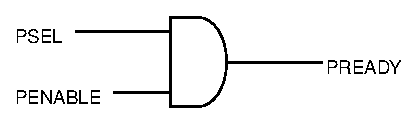
\includegraphics{figures/bloc_pready.eps}
\caption{A PREADY jel kombinációs logikája}
\label{fig:bloc_pready}
\end{center}
\vspace{0.5cm}
\end{figure}

Ha a megfelelő regiszter van címezve, akkor a perifériaillesztő adatot kell, hogy beolvasson az adatbuszról. A transmit modulban egy FIFO várja az új adatot, így ennek bemenetét kell engedélyezni a beolvasáshoz. A FIFO bemenetére \textit{(TxData)} így közvetlenül ráköthető az adatbusz alsó 8 bitje, és az engedélyező jelet \textit{(TxNext)}, pedig egy címzést vizsgáló logika adja. (\ref{fig:bloc_txdata}. és \ref{fig:bloc_txnext} ábra)

\begin{figure}[h]
\vspace{0.5cm}
\begin{center}
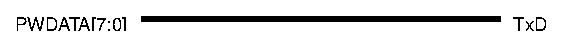
\includegraphics{figures/bloc_txdata.eps}
\caption{Küldendő adat továbbítása a transmit modulnak}
\label{fig:bloc_txdata}
\end{center}
\vspace{0.5cm}
\end{figure}
\begin{figure}[h]
\vspace{0.5cm}
\begin{center}
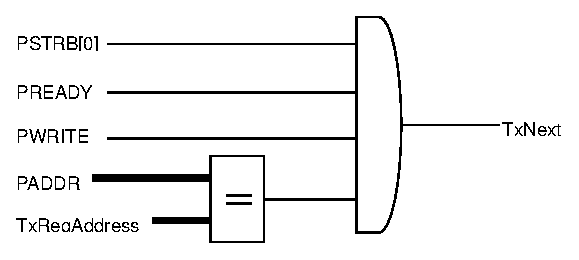
\includegraphics{figures/bloc_txnext.eps}
\caption{Új adat jelzése a transmit modulnak}
\label{fig:bloc_txnext}
\end{center}
\vspace{0.5cm}
\end{figure}

Hasonlóképpen kell jelezni az olvasást is, az \textit{RxNext} jelet a receive modul kapja meg, ahol a FIFO kimeneti engedélyező bemenetére van kapcsolva. (\ref{fig:bloc_rxnext}. ábra)

\begin{figure}[h]
\vspace{0.5cm}
\begin{center}
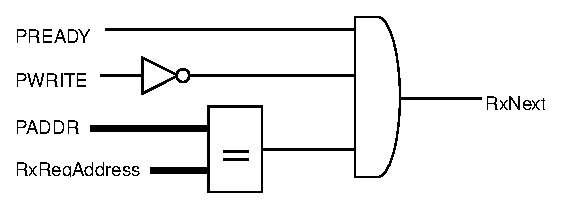
\includegraphics{figures/bloc_rxnext.eps}
\caption{Adat olvasásának jelzése a receive modulnak}
\label{fig:bloc_rxnext}
\end{center}
\vspace{0.5cm}
\end{figure}

Az APB buszra a címzés alapján hivatkozott regiszter tartalma kerül. Fontos, hogy ha a busz nem éppen a perifériaillesztőről olvas, akkor az ne hajtsa meg az adatbuszt. (\ref{fig:bloc_prdata}. ábra)

\begin{figure}[h]
\vspace{0.5cm}
\begin{center}
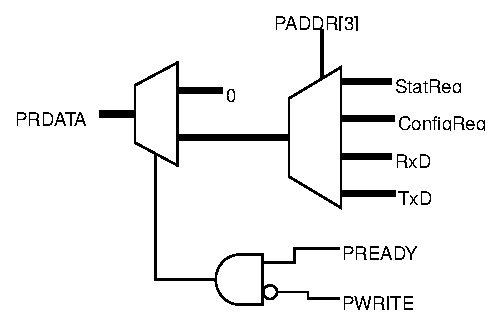
\includegraphics{figures/bloc_prdata.eps}
\caption{Buszra kerülő adatok}
\label{fig:bloc_prdata}
\end{center}
\vspace{0.5cm}
\end{figure}

A konfigurációs regiszternél meg kellett oldani, hogy csak a kívánt byteok módosuljanak a regiszter írásakor. A négybites \textit{PSTRB} bemenetből egy bitmaszkot hozunk létre, és ennek alapján töltjük be az új értéket, illetve tartjuk meg az előzőt. A regiszter engedélyező bemenetére egy címzési logikát kötöttünk. (\ref{fig:bloc_configreg}. ábra)

\begin{figure}[h]
\vspace{0.5cm}
\begin{center}
\includegraphics{figures/bloc_configreg.eps}
\caption{Konfigurációs regiszter beállítása}
\label{fig:bloc_configreg}
\end{center}
\vspace{0.5cm}
\end{figure}
\clearpage
\subsection{Transmit modul}
Az UART küldő modul logikailag különválasztható, így külön almodulként valósítjuk meg. Bemenetként megkapja a szükséges konfigurációs regiszterek értékeit, illetve a buszról érkező küldendő adatot. A fő modul felé jelzi, ha a FIFO tele van, vagy üres, illetve az UART kimenet közvetlenül az egész perifériaillesztő kimenete is.

A transmit modul egy állapotgép alapján működik. (\ref{fig:tx_state}. ábra) A megfelelő baud rate-et a \textit{BCount} számlálóval érjük el, ami a konfiguráció alapján kiszámolt végértéknél lépteti az állapotgépet. A kimeneti regiszter \textit{(shMem)} értékének betöltését az ábrán \textit{shMem.load}-dal jelöltük, ennek értéke a küldendő adat, kiegészítve a megfelelő start és stop bitekkel. 0-tól különböző állapot esetén az UART kimenetre ennek a regiszternek az állapot számával címzett bitje kerül.

\begin{figure}[h]
\vspace{0.5cm}
\begin{center}
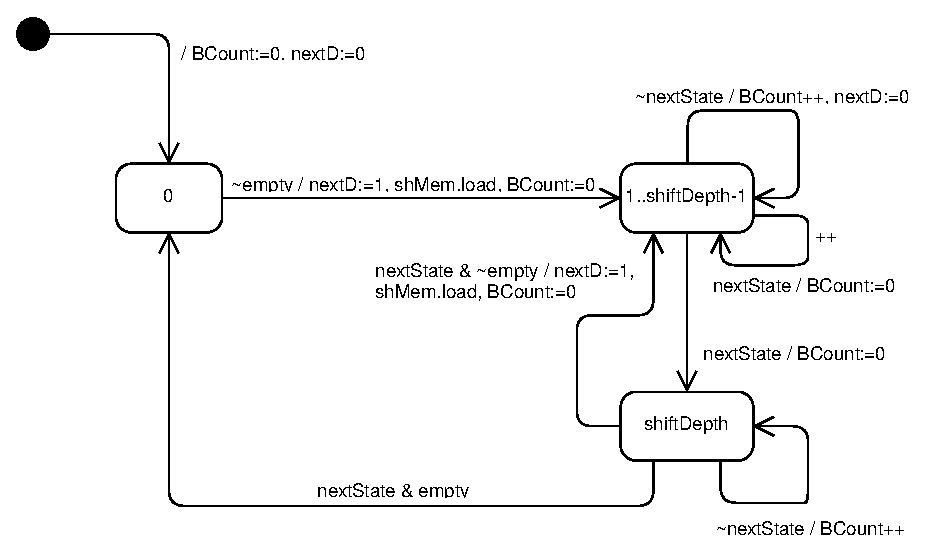
\includegraphics{figures/tx_state.eps}
\caption{A küldő modul állapotgépe}
\label{fig:tx_state}
\end{center}
\vspace{0.5cm}
\end{figure}

\textit{Rst} jelre a modul \textit{0} állapotba kerül, ez az állapot jelenti az UART küldés felfüggesztését. Ha a FIFO nem üres, a kimeneti regiszterbe bekerül belőle egy adat (a \textit{nextD} jel kivesz a FIFO-ból egy elemet), és az állapotgép 1-es állapotba kerül. Az állapotok 1-től \textit{shiftDepth}-ig (ami a konfiguráció alapján a kimeneti regiszter adatmérete). Az utolsó bit után az állapotgép újraindul, ha a FIFO-ban van még adat, illetve 0-ás állapotba kerül, ha nincs. 0-ás állapotban a kimenet magasban van (nincs adat).

\begin{figure}[h]
\vspace{0.5cm}
\begin{center}
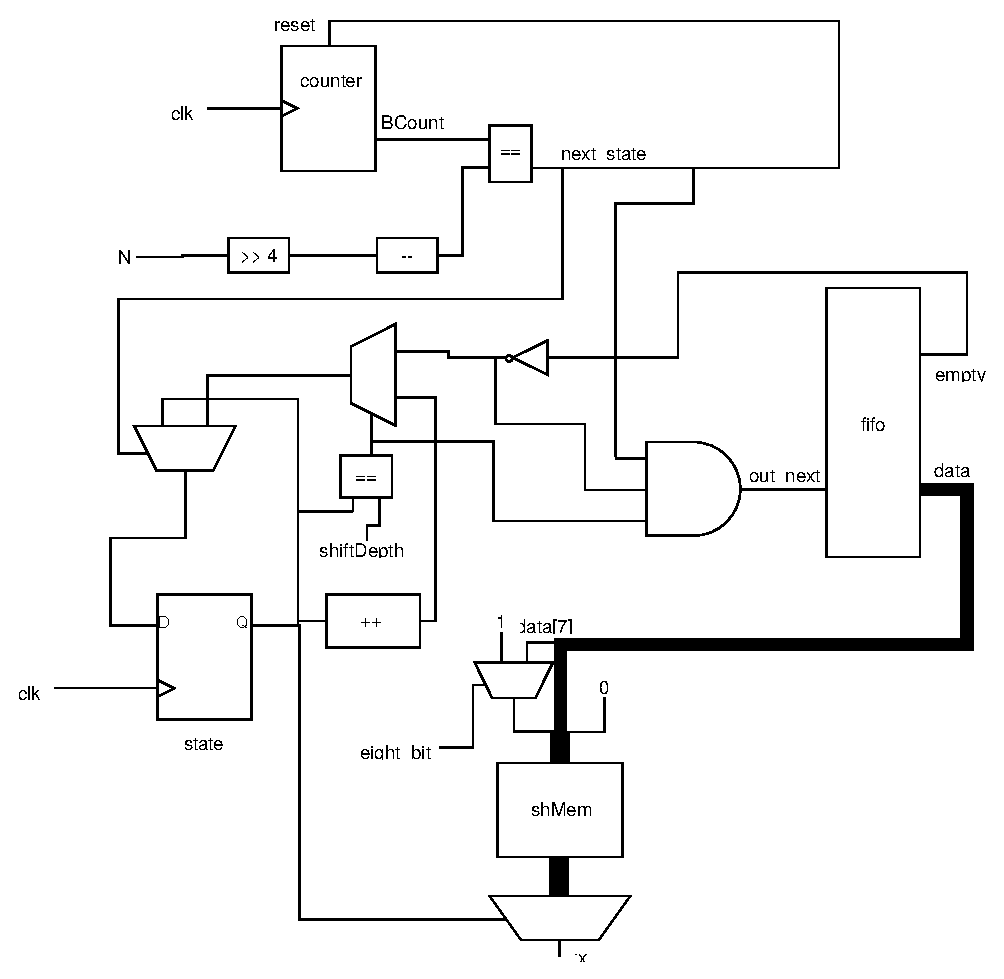
\includegraphics{figures/transmit.eps}
\caption{A küldő modul blokkdiagramja}
\label{fig:transmit}
\end{center}
\vspace{0.5cm}
\end{figure}

\clearpage
\subsection{Receive modul}
A fogadó modul egy hasonló állapotgéppel működik, mint a küldő, az állapotok itt is az egyes bitek helyét kódolják a byteon belül. A modul \textit{SClk} órajellel vesz mintát az UART bemenetről, ez az órajel az APB órajel N-ed része (ld. konfigurációs regiszter), a baud rate 16-szorosa. Az állapotgép kezdő állapota a 0, ez jelenti, hogy a fogadó a start bitre vár. Ekkor alacsony jel észlelésekor vár fél bitidőt, és ha a jel ezalatt mindvégig alacsony, akkor elindul az állapotgép, és a konfigurációnak megfelelően beolvassa a byteot. A \textit{shMem} regiszterbe a bemenet egy többségi szavazással (\ref{fig:voter}. ábra) beolvasott értéke kerül, a bitidő közepéről mintavételezve.

\begin{figure}[h]
\vspace{0.5cm}
\begin{center}
\includegraphics{figures/voter.eps}
\caption{A beérkezett bit többségi szavazással beolvasva}
\label{fig:voter}
\end{center}
\vspace{0.5cm}
\end{figure}

\clearpage
\section{Megvalósítás}

\begin{lstlisting}[frame=single,language=verilog,caption={APB UART top modul},captionpos=b,label={lst:apb}]
module APB_UART(
    output Tx,
    input Rx,
    input PCLK,
    input PRESETn,
    input [31:0] PADDR,
    input PSEL,
    input PENABLE,
    input PWRITE,
    input [31:0] PWDATA,
    input [3:0] PSTRB,
    output PREADY,
    output [31:0] PRDATA
    );
    
    assign PREADY = (PSEL & PENABLE);
    
    wire TxNext, TxEmpty, TxFull;
    assign TxNext = (PSTRB[0] & PREADY & PWRITE & (PADDR == 32'd12));
    transmitter tr (
        .clk(PCLK),
        .rst(!PRESETn),
        .N(confg[15:0]),
        .eight_bit(confg[16]),
        .two_stop(confg[17]),
        .data(PWDATA[7:0]),
        .next(TxNext),
        .Tx(Tx),
        .empty(TxEmpty),
        .full(TxFull)
        );
    
    wire [7:0] RxData;
    wire RxNext, RxEmpty, RxFull;
    assign RxNext = (PREADY & !PWRITE & (PADDR == 32'd8));
    receiver rec(
        .clk(PCLK),
        .rst((!PRESETn) || (!confg[18])), //hold in reset if disabled
        .N(confg[15:0]),
        .eight_bit(confg[16]),
        .Rx(Rx),
        .data(RxData),
        .next(RxNext),
        .empty(RxEmpty),
        .full(RxFull)
        );
    
    reg [18:0] confg;
    wire confg_en;
    wire [18:0] M;
    assign M = {{3{PSTRB[2]}}, {8{PSTRB[1]}}, {8{PSTRB[0]}}};
    assign confg_en = (PREADY & PWRITE & (PADDR == 32'd0));
    always @(posedge PCLK) begin
        if(!PRESETn)
            confg <= {3'b001, 16'd100}; //defaults: 8N1, receiver disabled, baud=62'500
        else begin
            if(confg_en) begin
                confg <= ((confg & (~M)) | (PWDATA[18:0] & M)); //confg[n]:=(confg[n-1]*~M)+(PWDATA*M) -> only changes the bytes which are set in PSTRB
            end
        end
    end
    
    wire [31:0] mux;
    assign mux = (
        (PADDR == 32'd0) ? ({13'd0, confg}) : (
            (PADDR == 32'd4) ? ({16'd0, {6'b0, RxFull, RxEmpty}, {6'b0, TxFull, TxEmpty}}) : (
                (PADDR == 32'd8) ? ({24'd0, RxData}) : (
                    32'd0 //deafult choise
                    )
                )
            )
        );
    
    assign PRDATA = ((PREADY && (!PWRITE)) ? mux : 32'd0);
endmodule
\end{lstlisting}

\begin{lstlisting}[frame=single,language=verilog,caption={Receive modul},captionpos=b,label={lst:recv}]
module receiver(
    input clk,
    input rst,
    input [15:0] N, //f_sampling = F_osc / N = 16 * baud
    input eight_bit,
    input Rx,
    output [7:0] data,
    input next,
    output empty,
    output full
    );
        
    wire SClk;
    reg [15:0] SClk_count;
    assign SClk = (N == 16'd1) ? clk : (SClk_count == N-1);
    always @(posedge clk) begin
        if(rst)
            SClk_count <= 0;
        else if(SClk)
             SClk_count <= 0;
        else
            SClk_count <= SClk_count + 1;            
    end
    
    reg sample;
    always @(posedge clk)
        if(SClk)
            sample <= Rx;
    
    reg buff[1:0];
    wire dec;
    assign dec = ((sample + buff[0] + buff[1]) >= 2'd2); 
    always @(posedge clk) begin
        if(SClk) begin
            buff[0] <= buff[1];
            buff[1] <= sample;
        end
    end
    
    reg [7:0] shMem;
    reg rec;
    FIFO #(.depth(32)) mem(
        .clk(clk),
        .rst(rst),
        .in(shMem),
        .in_next(rec),
        .out(data),
        .out_next(next),
        .empty(empty),
        .full(full)
        );
    
       
    reg [3:0] state; //0:wait, 1:start bit, 2-:data bits
    reg [3:0] cnt;
    always @(posedge clk) begin
        if(rst) begin
            state <= 4'd0;
            rec <= 1'b0;
        end
        else if(SClk) begin
            if(state == 4'd0) begin
                if(sample == 1'b0) begin //start condition
                    state <= 4'd1;
                    cnt <= 4'd0;
                end
			end
            else if(state == 4'd1) begin
                if(sample == 1'b1)
                    state <= 4'd0;
                else begin
                    if(cnt == 8) begin //if the start condition lasted for half a bit time + 1 sample (so that subsequent bits will be sampled at the middle)
                        cnt <= 4'd0;
                        state <= state + 1;
                    end
                    else
                        cnt <= cnt + 1;
                end
            end
            else if(state == (4'd8 + eight_bit)) begin //last bit
                if(cnt == 4'd15) begin
                    state <= 4'd0;
                    shMem[state - 4'd2] <= dec;
                    rec <= 1'b1;
                end
                else
                    cnt <= cnt + 1;
            end
            else begin
                if(cnt == 4'd15) begin
                    cnt <= 4'd0;
                    state <= state + 4'd1;
                    shMem[state - 4'd2] <= dec;
                end
                else
                    cnt <= cnt + 1;
            end
        end
        else
            rec <= 1'b0;
    end
    
endmodule
\end{lstlisting}

\begin{lstlisting}[frame=single,language=verilog,caption={Transmit modul},captionpos=b,label={lst:trmt}]
module transmitter(
    input clk,
    input rst,
    input [15:0] N, //f_sampling = F_osc / N = 16 * baud
    input eight_bit,
    input two_stop,
    output empty,
    output full,
    input [7:0] data,
    input next,
    output Tx
    );
        
    wire [7:0] D;
    reg nextD;
    FIFO #(.depth(32)) mem(
        .clk(clk),
        .rst(rst),
        .in(data),
        .in_next(next),
        .out(D),
        .out_next(nextD),
        .empty(empty),
        .full(full)
        );
    
    reg [10:0] shMem;    
    reg [3:0] state; //0: wait, 1 - 1+bit_num+stop_num: send
    reg [19:0] BCount;
    wire nextState;
    assign nextState = (BCount == ({N, 4'd0} - 1));
    wire [3:0] shiftDepth;
    assign shiftDepth = (4'd1 + 4'd7 + {3'd0, eight_bit} + 4'd1 + {3'd0, two_stop}); //start_bit + 7_data_bits + eight_bit + stop_bit + 2nd_stop_bit
    assign Tx = (state == 4'd0) ? 1'b1 : shMem[state - 4'd1];
    
    always @(posedge clk) begin
        if(rst) begin
            BCount <= 0;
            state <= 0;
            nextD <= 0;
        end
        else begin
            if(state == 0) begin
                if(!empty) begin
                    nextD <= 1;
                    shMem <= {2'b11, (eight_bit ? D[7] : 1'b1), D[6:0], 1'b0}; //11 - eight_bit or stop bit - data - start bit
                    state <= 4'd1;
                    BCount <= 19'd0;
                end
            end
            else begin
                if(state == shiftDepth) begin
                    if(nextState) begin
                        if(!empty) begin
                            nextD <= 1;
                            shMem <= {2'b11, (eight_bit ? D[7] : 1'b1), D[6:0], 1'b0}; //11 - eight_bit or stop bit - data - start bit
                            state <= 4'd1;
                            BCount <= 19'd0;
                        end
                        else
                            state <= 4'd0;
                    end
                    else begin
                        BCount <= BCount + 1;
                    end
                end
                else begin
                    if(nextState) begin
                        state <= state + 1;
                        BCount <= 19'd0;
                    end
                    else begin
                        BCount <= BCount + 1;
                        nextD <= 0;
                    end
                end
            end
            
        end
    end
    
endmodule
\end{lstlisting}
\begin{lstlisting}[frame=single,language=verilog,caption={FIFO verilog modul},captionpos=b,label={lst:fifo}]
module FIFO #(parameter depth = 32)(
    input clk,
    input rst,
    input [7:0] in,
    input in_next,
    output [7:0] out,
    input out_next,
    output empty,
    output full
    );
    
    reg [$clog2(depth+1)-1:0]count;
    reg [7:0] mem [depth-1:0];
    
    assign empty = (count == 0);
    assign full = (count == depth);
    assign out = mem[0];
    
    integer ii;
    always @(posedge clk) begin
        if(rst)
           count <= 0;
        else begin            
            if(in_next && !out_next) begin //write
                count <= count + 1;
                mem[count] <= in;
            end
            
            if(!in_next && out_next) begin //read
                count <= count - 1;
                for(ii = 0; ii < (depth-1); ii = ii + 1 )
                    mem[ii] <= mem[ii+1];
            end
            
            if(in_next && out_next) begin //write and read
                mem[count] = in;                
                for(ii = 0; ii < (depth-1); ii = ii + 1 )
                    mem[ii] <= mem[ii+1];
            end
        end
    end
    
endmodule
\end{lstlisting}
\section{Tesztelés}
\begin{figure}[h]
\begin{center}
\includegraphics[height=4cm]{figures/test.png}
\caption{Szimulációs jelalak}
\label{fig:Testsim}
\end{center}
\end{figure}

